
%(BEGIN_QUESTION)
% Copyright 2006, Tony R. Kuphaldt, released under the Creative Commons Attribution License (v 1.0)
% This means you may do almost anything with this work of mine, so long as you give me proper credit

Displacer-type instruments are often used to measure liquid level:

$$\includegraphics[width=15.5cm]{i00280x01.eps}$$

How might such an instrument be modified to measure liquid {\it density} instead?

\vskip 20pt \vbox{\hrule \hbox{\strut \vrule{} {\bf Suggestions for Socratic discussion} \vrule} \hrule}

\begin{itemize}
\item{} A problem-solving technique to employ here is examining the buoyant force equation to identify which physical quantities are fixed and which are variable in a standard level-measuring instrument, then asking ourselves which quantities would have to be fixed versus variable to turn this into a {\it density}-measuring instrument.  Explore this technique to see if this helps you answer the question.
\end{itemize}

\underbar{file i00280}
%(END_QUESTION)





%(BEGIN_ANSWER)


%(END_ANSWER)





%(BEGIN_NOTES)

In order to measure density with a displacer-type instrument, it would have to be arranged in such a way that it always remained {\it full} of liquid.  Then, only changes in liquid density would affect the displacer's weight.  I'll let you think of ways to do this!

\vskip 10pt

One way to ensure total immersion of the displacer is to do this:

$$\includegraphics[width=15.5cm]{i00280x02.eps}$$

Of course, the sample flow rate must be limited enough that any dynamic forces on the displacer are negligible.

%INDEX% Measurement, density: displacer (buoyancy)

%(END_NOTES)


